a. Run this program for each method and produce a plot similar to Figure 4.1.\\
b. The convergence behavior of SOR is very sensitive to the choice of $\omega$. Try changing from the
optimal $\omega$ to $\omega=1.8$ or $1.95$.\\
c. Let $g(\omega)=\rho(G(\omega))$ be the spectral radius of the iteration matrix $G$ for a given value
of $\omega$. Write a program to produce a plot of $g(\omega)$ for $0\leq\omega\leq2$.\\
d. Try this computationally and observe that it does not work well. Explain what is wrong with this and
derive the correct expression (4.24).\\

\begin{solution}\renewcommand{\qedsymbol}{}\ \\ 
    \begin{center}
        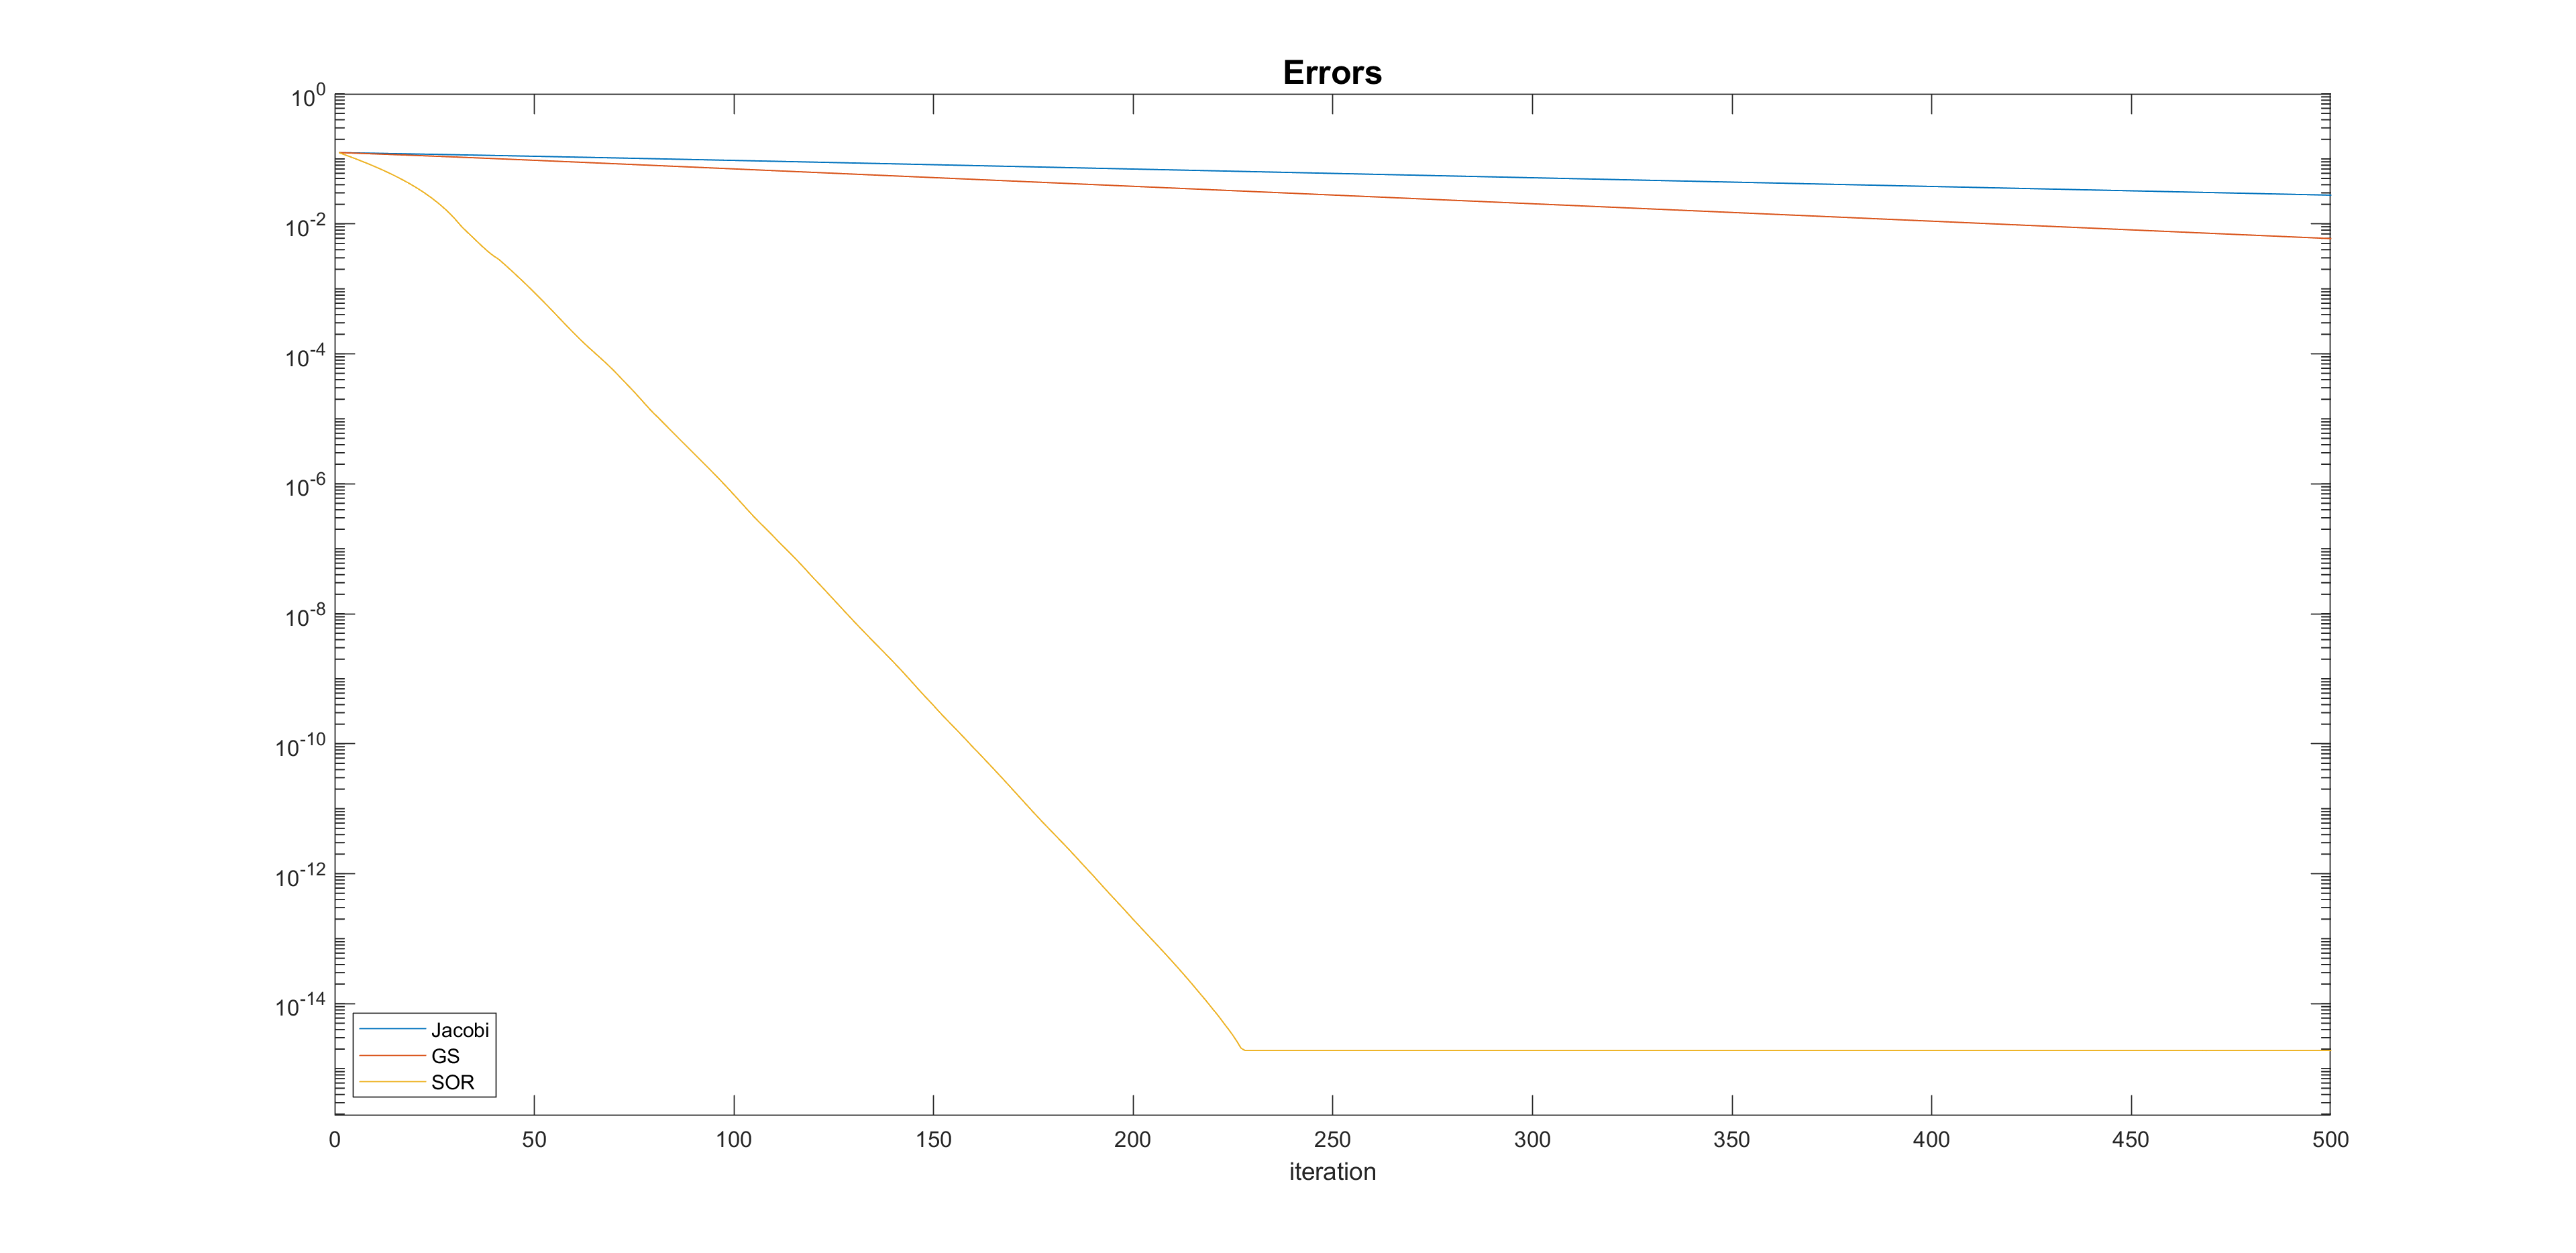
\includegraphics[scale=0.15]{vs.PNG}
    \end{center}
    \begin{center}
        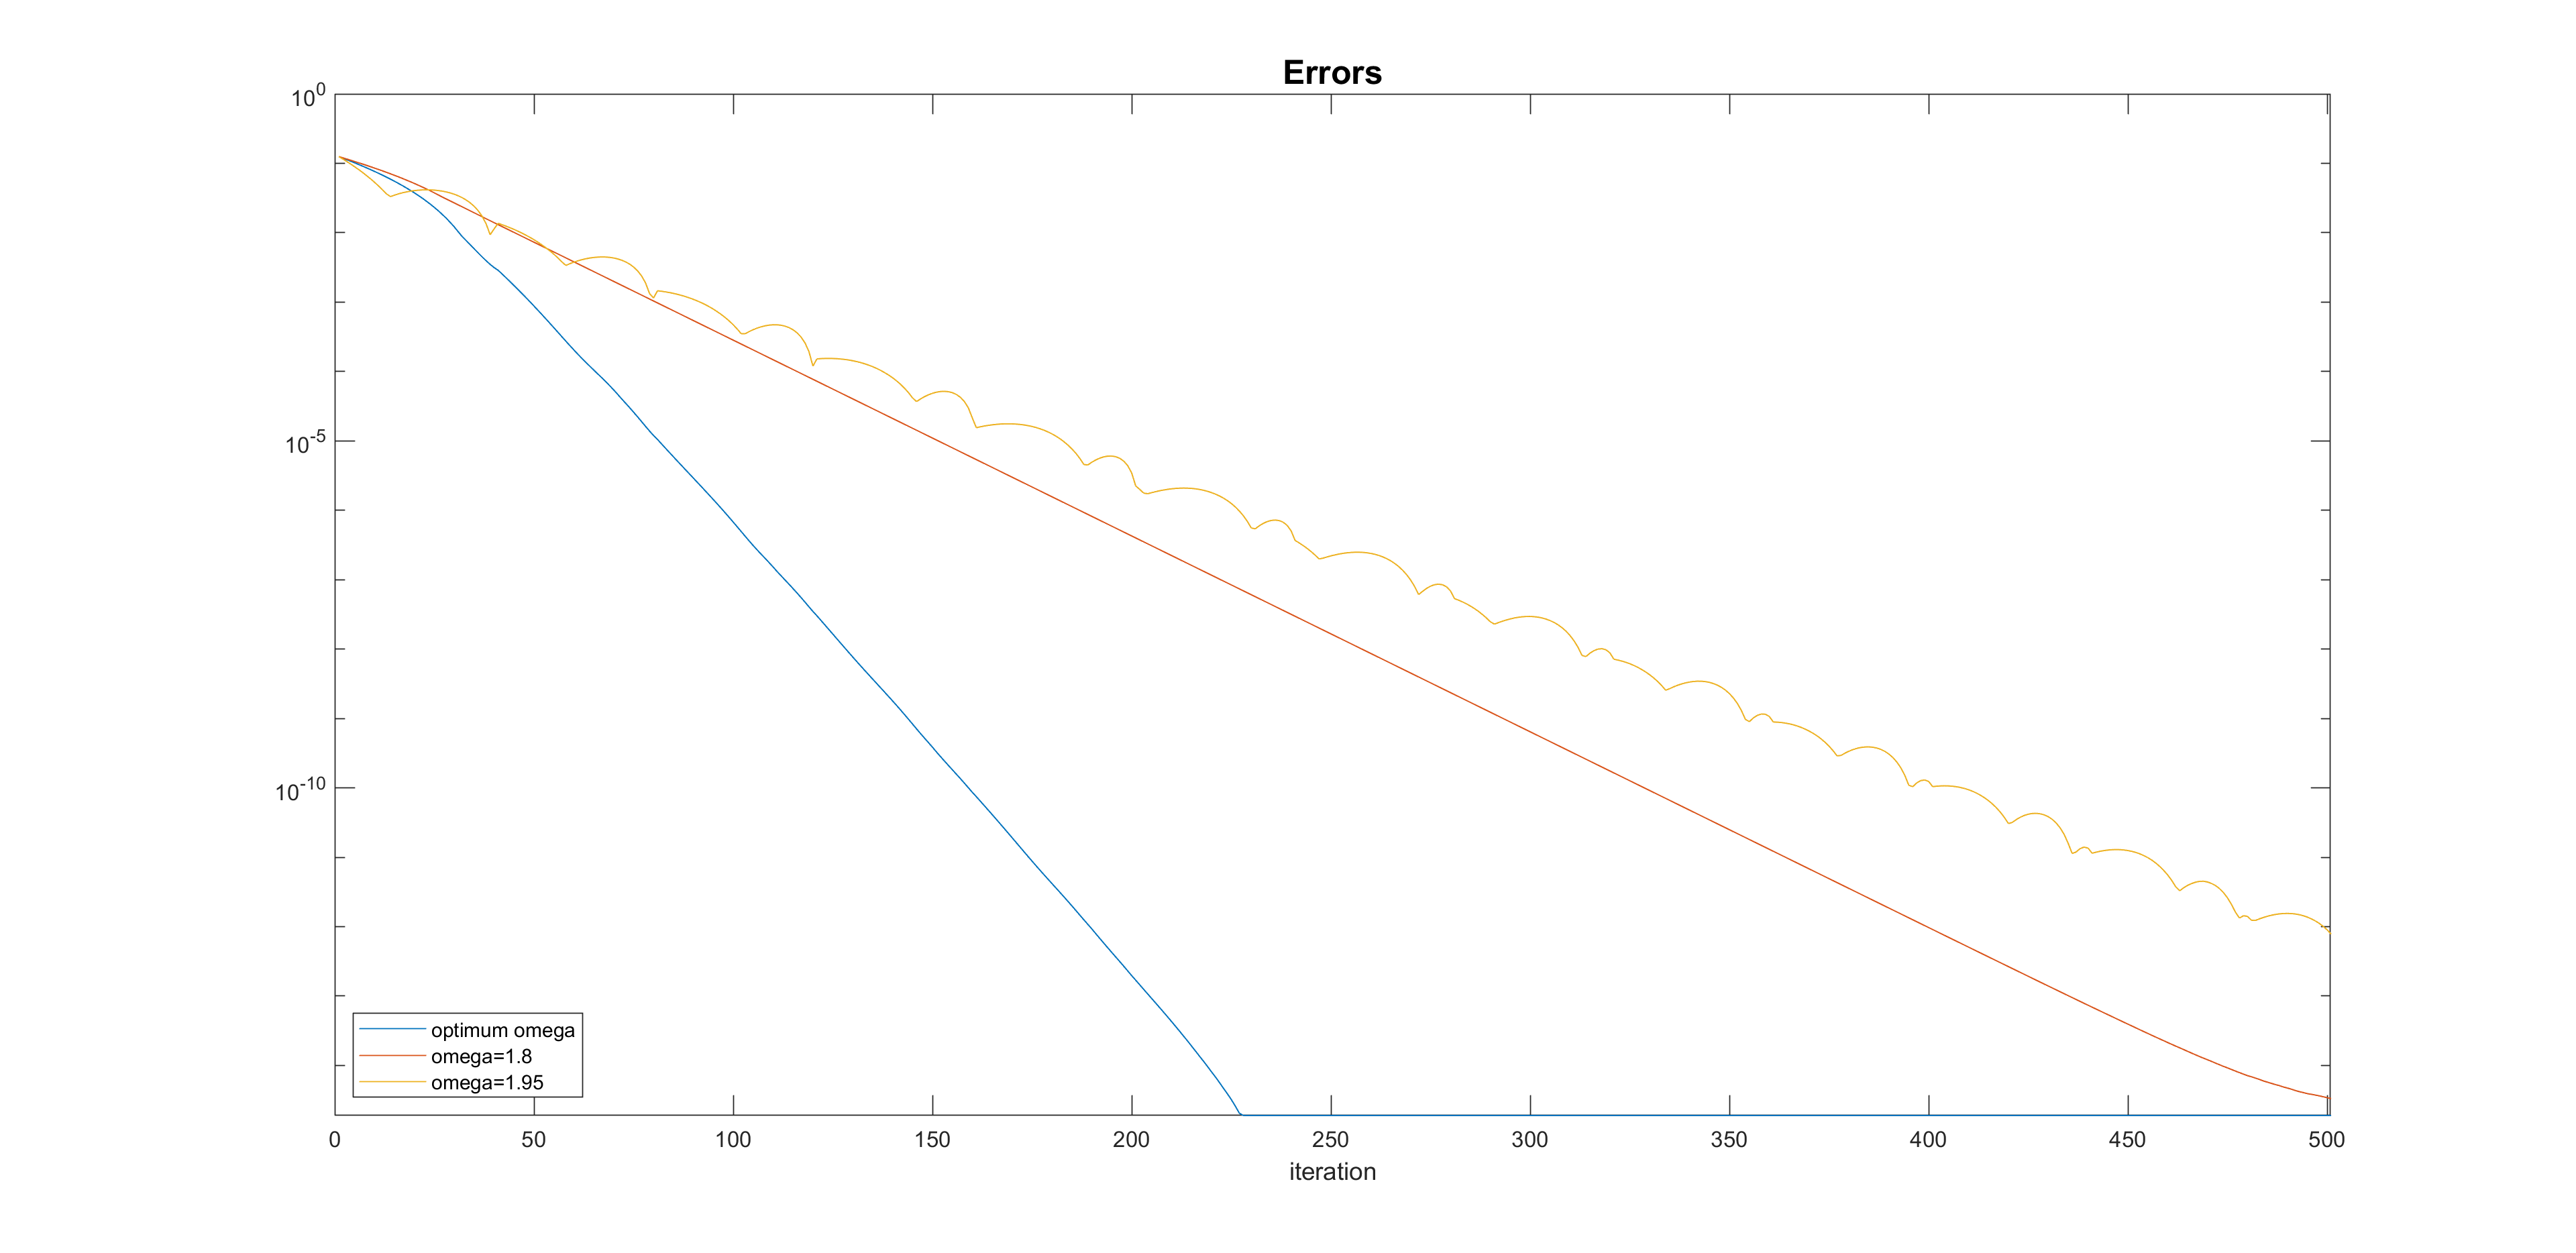
\includegraphics[scale=0.15]{omega.PNG}
    \end{center}
    \begin{center}
        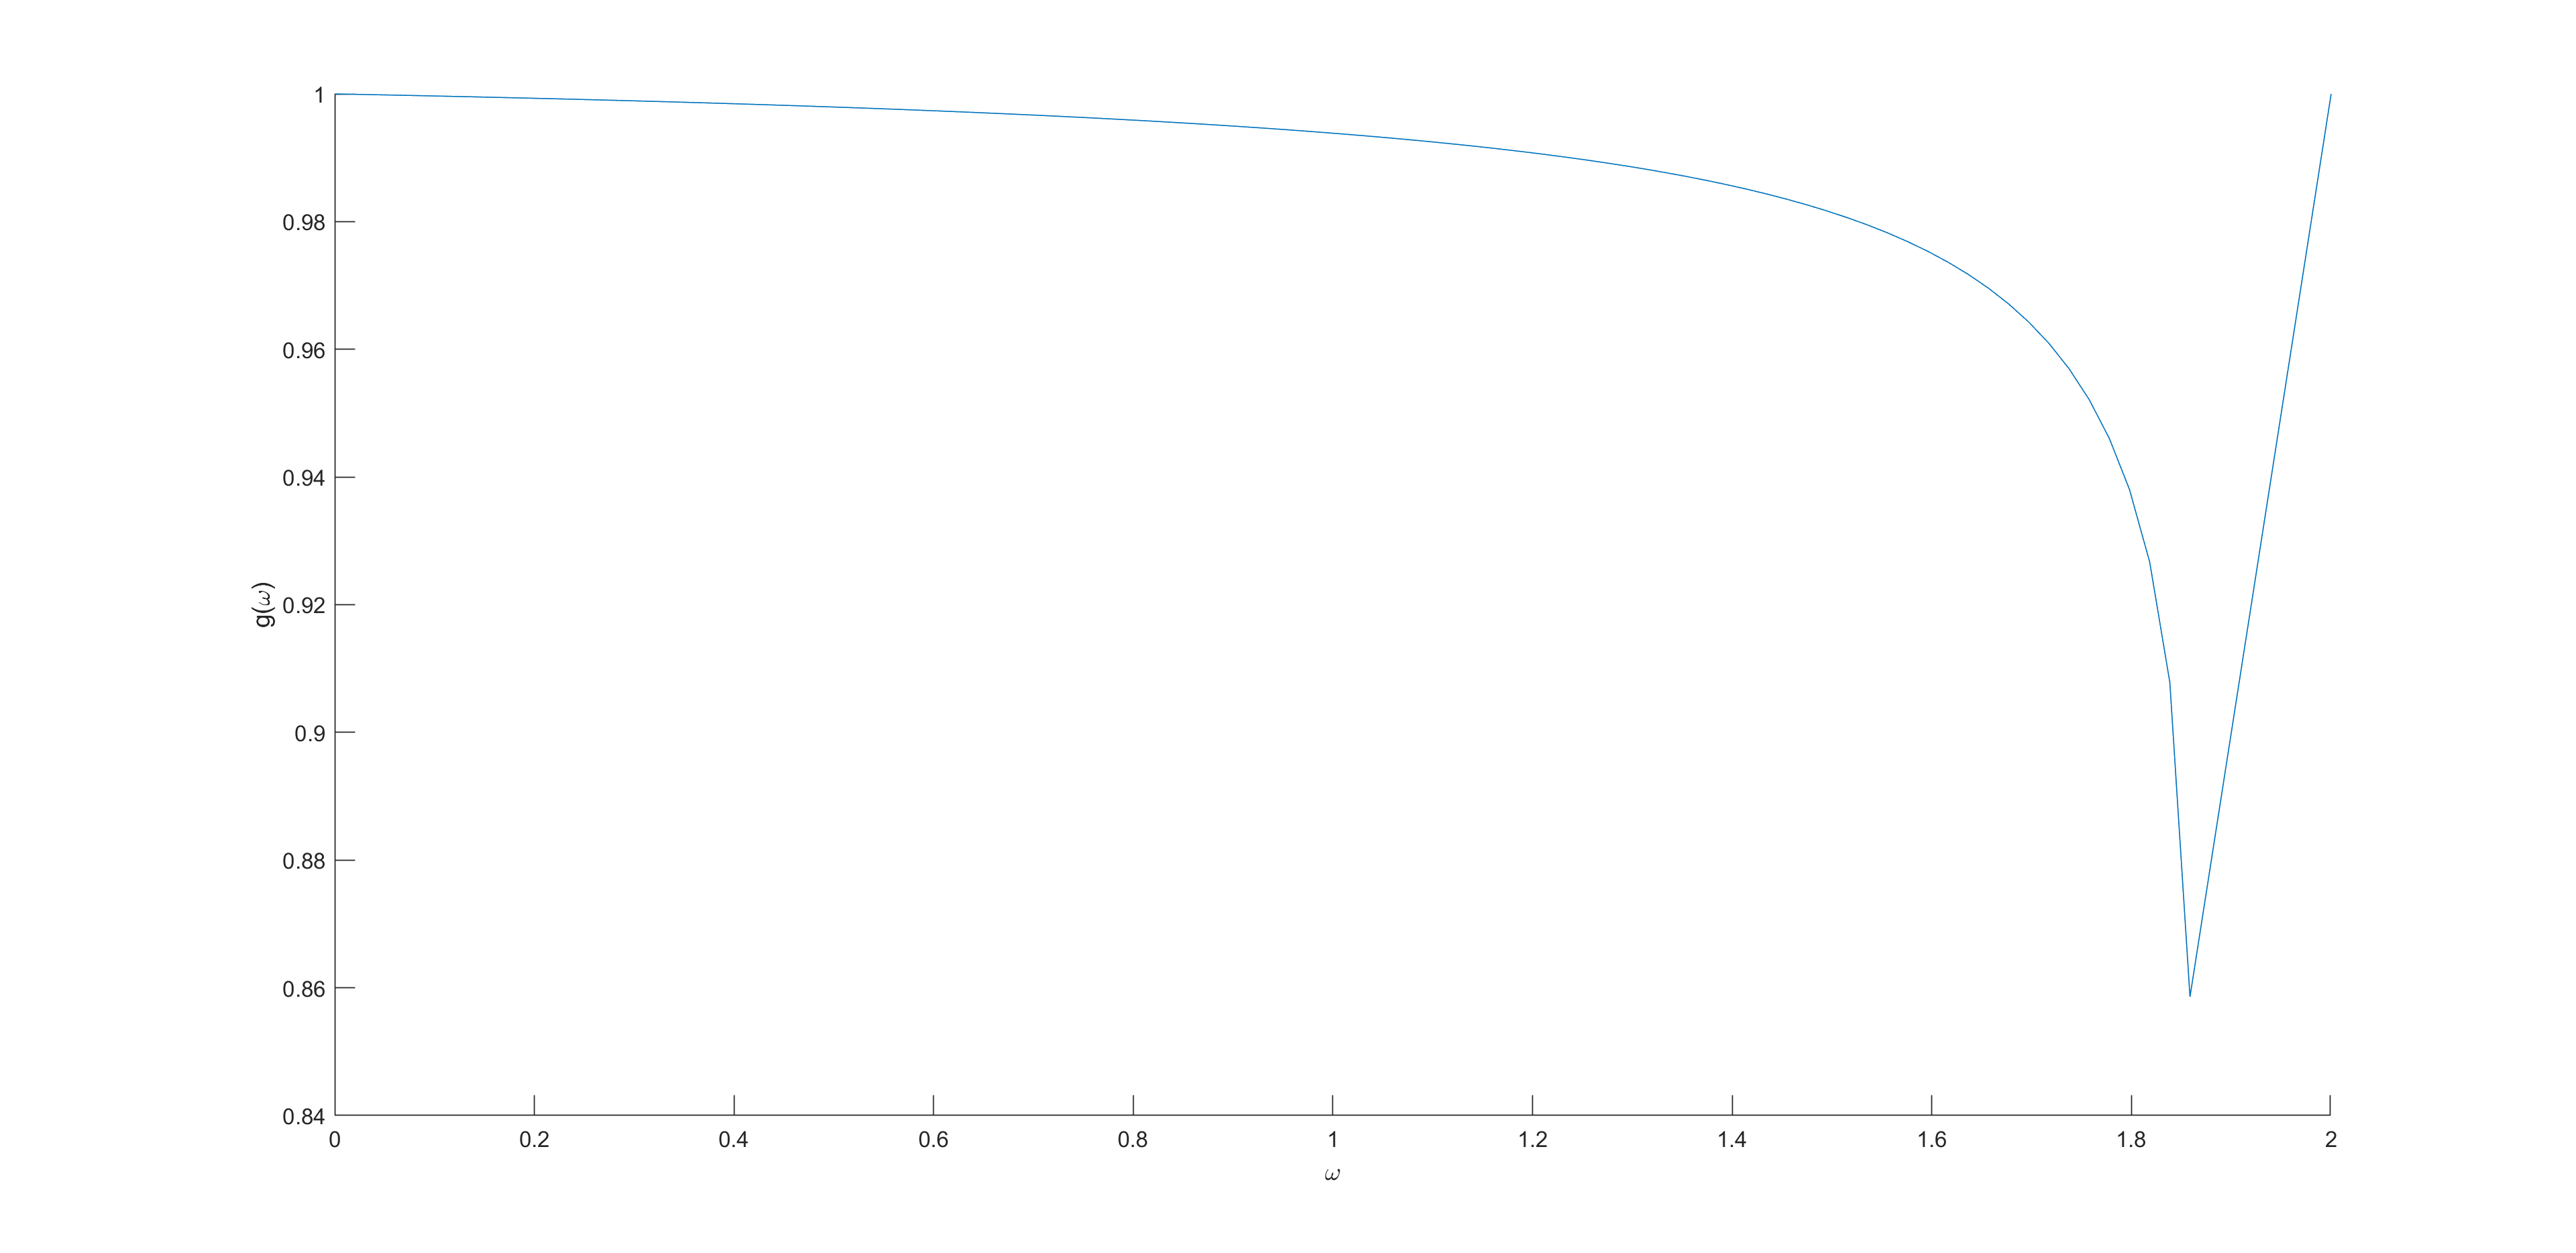
\includegraphics[scale=0.15]{omegaiter.PNG}
    \end{center}

    We see by the figure below that this method clearly does not work well. Given that the true solution
    was supposed to be a second order polynomial, this na\"ive SOR method does not hold.

    \begin{center}
        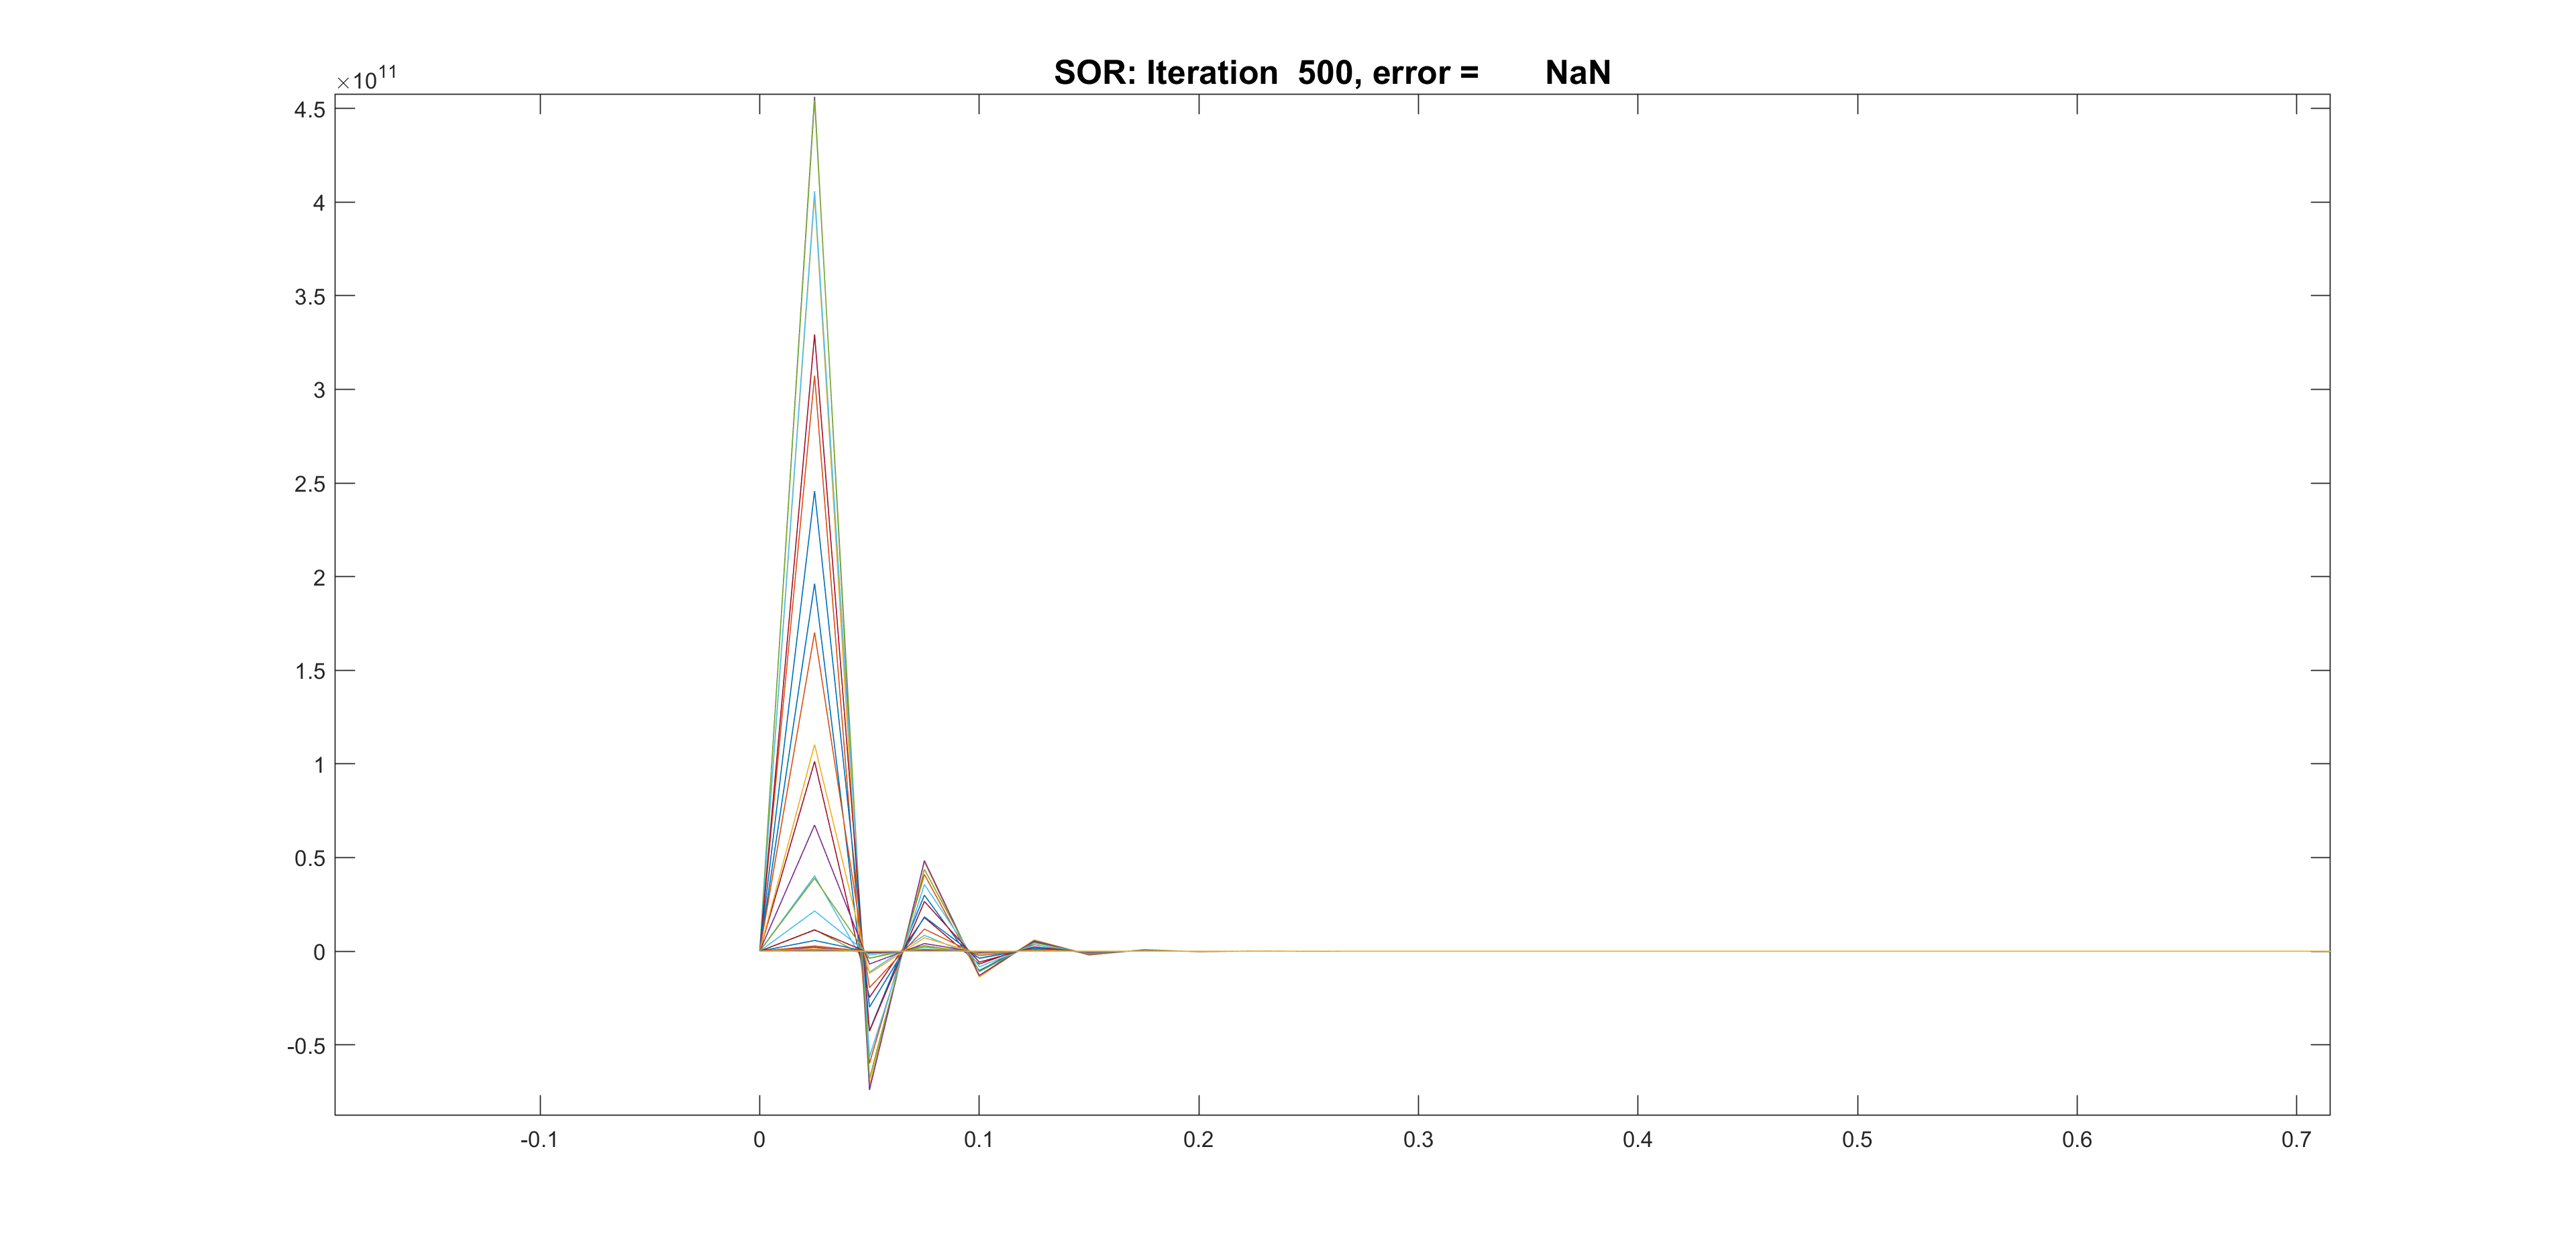
\includegraphics[scale=0.15]{badsor.PNG}
    \end{center}

    Now, starting from equations (2.22), we have

    $$u^{GS}_i=\frac12(u^{[k+1]}_{i-1}+u^{[k]}_{i+1}-h^2f_i)$$

    $$u^{[k+1]}_i=u^{[k]}_i+\omega(u^{GS}_i-u^{[k]}_i)$$

    Hence,

    $$u^{[k+1]}_i=u^{[k]}_i+\omega(\frac12((u^{[k+1]}_{i-1}+u^{[k]}_{i+1}-h^2f_i)-u^{[k]}_i))=$$
    $$u^{[k]}_i-\omega u^{[k]}_i+\frac{\omega}{2}(u^{[k+1]}_{i-1}+u^{[k]}_{i+1}-h^2f_i)=
    (1-\omega)u^{[k]}_i+\frac{\omega}{2}(u^{[k+1]}_{i-1}+u^{[k]}_{i+1}-h^2f_i)$$

    So. we have that

    $$u^{[k+1]}_i=(1-\omega)Du^{[k]}+\frac{\omega}{2}(Lu^{[k+1]}+Uu^{[k]}-h^2f_i)$$
    $$\omega\frac{1}{\omega}((1-\omega)D+\frac{\omega}{2}U)u^{[k]}+\frac{\omega}{2}Lu^{[k+1]}
    -\frac{h^2\omega}{2}f_i$$
    
    Therefore, we see that

    $$M=\frac{1}{\omega}(D-\omega L)\;\text{and}\;N=\frac{1}{\omega}((1-\omega)D+\omega U)$$

\end{solution}